\section{任务五}

\subsection{PHILOX-2W的一轮差分传播}
按照实验指导书中的公式，定义
\[
    \operatorname{mulhi}_M(X)
    =\left\lfloor\frac{X\cdot M}{2^W}\right\rfloor,
    \qquad
    \operatorname{mullo}_M(X)
    =(X\cdot M)\bmod 2^W.
\]
其中每个分支为 $W$ 比特，$M$ 为固定常数，$K$ 为一轮子密钥。PHILOX-2W的一轮变换为
\[
    L'=\operatorname{mulhi}_M(R),
    \qquad
    R'=\operatorname{mullo}_M(R)\oplus L\oplus K.
\]
设一对输入为 $(L_1,R_1)$ 和 $(L_2,R_2)$，其输入差分为
\[
    \Delta L=L_1\oplus L_2,
    \qquad
    \Delta R=R_1\oplus R_2.
\]
因此可令 $L_2=L_1\oplus\Delta L$、$R_2=R_1\oplus\Delta R$。经过一轮变换后，左分支输出差分为
\[
\begin{aligned}
    \Delta L'
    &=L_1'\oplus L_2'\\
    &=\operatorname{mulhi}_M(R_1)
      \oplus\operatorname{mulhi}_M(R_1\oplus\Delta R),
\end{aligned}
\]
右分支输出差分为
\[
\begin{aligned}
    \Delta R'
    &=R_1'\oplus R_2'\\
    &=\operatorname{mullo}_M(R_1)\oplus L_1\oplus K \oplus\operatorname{mullo}_M(R_1\oplus\Delta R)
      \oplus L_1\oplus\Delta L\oplus K\\
    &=\operatorname{mullo}_M(R_1)
      \oplus\operatorname{mullo}_M(R_1\oplus\Delta R)
      \oplus\Delta L.
\end{aligned}
\]
可见，相同的轮密钥 $K$ 在差分中抵消。给定输入差分后，输出差分只需遍历 $R_1$ 的取值即可确定；对每个 $R_1$，所有 $2^W$ 个 $L_1$ 都产生相同的输出差分。
当 $\Delta R=0$ 时，两次乘法输入相同，乘积高、低字的差分均为零，因此
\[
    (\Delta L,0)\longrightarrow(0,\Delta L)
\]
以概率 $1$ 发生。特别地，输入差分 $(\texttt{0x}01,\texttt{0x}00)$ 必然传播为输出差分 $(\texttt{0x}00,\texttt{0x}01)$。

\subsection{程序与参数}

程序按照上述一轮公式实现 $\operatorname{mulhi}_M$、$\operatorname{mullo}_M$ 和轮变换，并对全部 $2^{2W}=2^{16}$ 个输入状态 $(L,R)$ 进行穷举。对于每种输入差分，输出差分的出现概率按其计数除以 $2^{16}$ 计算。实验参数为
\[
    W=8,\qquad M=\texttt{0x}9B,\qquad K=\texttt{0x}46.
\]
代码对同一输入对使用相同的轮密钥 $K=\texttt{0x}46$。由于 $K$ 在差分中抵消，轮密钥取值不会改变统计分布。程序分别统计输入差分
$(\texttt{0x}00,\texttt{0x}01)$、
$(\texttt{0x}01,\texttt{0x}00)$、
$(\texttt{0x}00,\texttt{0x}02)$ 和
$(\texttt{0x}02,\texttt{0x}01)$，并列出每种情况概率最高的五个输出差分。
\subsection{实验结果}

表中概率由完整的 $2^{16}$ 个输入状态穷举得到；若多个输出差分的计数相同，则按输出差分数值升序排列。

\begin{table}[H]
    \centering
    \small
    \caption{PHILOX-2W一轮变换的高频输出差分}
    \label{tab:task5_top_differences}
    \renewcommand{\arraystretch}{1.1}
    \begin{tabular}{cccrr}
        \toprule
        输入差分 $(\Delta L,\Delta R)$ & 排名 & 输出差分 $(\Delta L',\Delta R')$ & 计数 & 概率 \\
        \midrule
        $(\texttt{0x}00,\texttt{0x}01)$ & 1 & $(\texttt{0x}00,\texttt{0x}9B)$ & 4096 & 0.0625000000 \\
        $(\texttt{0x}00,\texttt{0x}01)$ & 2 & $(\texttt{0x}00,\texttt{0x}A7)$ & 4096 & 0.0625000000 \\
        $(\texttt{0x}00,\texttt{0x}01)$ & 3 & $(\texttt{0x}00,\texttt{0x}AB)$ & 4096 & 0.0625000000 \\
        $(\texttt{0x}00,\texttt{0x}01)$ & 4 & $(\texttt{0x}01,\texttt{0x}9B)$ & 2560 & 0.0390625000 \\
        $(\texttt{0x}00,\texttt{0x}01)$ & 5 & $(\texttt{0x}01,\texttt{0x}A7)$ & 2560 & 0.0390625000 \\
        \midrule
        $(\texttt{0x}01,\texttt{0x}00)$ & 1 & $(\texttt{0x}00,\texttt{0x}01)$ & 65536 & 1.0000000000 \\
        \midrule
        $(\texttt{0x}00,\texttt{0x}02)$ & 1 & $(\texttt{0x}01,\texttt{0x}4A)$ & 4096 & 0.0625000000 \\
        $(\texttt{0x}00,\texttt{0x}02)$ & 2 & $(\texttt{0x}01,\texttt{0x}36)$ & 3072 & 0.0468750000 \\
        $(\texttt{0x}00,\texttt{0x}02)$ & 3 & $(\texttt{0x}01,\texttt{0x}4E)$ & 2560 & 0.0390625000 \\
        $(\texttt{0x}00,\texttt{0x}02)$ & 4 & $(\texttt{0x}02,\texttt{0x}CA)$ & 2560 & 0.0390625000 \\
        $(\texttt{0x}00,\texttt{0x}02)$ & 5 & $(\texttt{0x}01,\texttt{0x}3A)$ & 2048 & 0.0312500000 \\
        \midrule
        $(\texttt{0x}02,\texttt{0x}01)$ & 1 & $(\texttt{0x}00,\texttt{0x}99)$ & 4096 & 0.0625000000 \\
        $(\texttt{0x}02,\texttt{0x}01)$ & 2 & $(\texttt{0x}00,\texttt{0x}A5)$ & 4096 & 0.0625000000 \\
        $(\texttt{0x}02,\texttt{0x}01)$ & 3 & $(\texttt{0x}00,\texttt{0x}A9)$ & 4096 & 0.0625000000 \\
        $(\texttt{0x}02,\texttt{0x}01)$ & 4 & $(\texttt{0x}01,\texttt{0x}99)$ & 2560 & 0.0390625000 \\
        $(\texttt{0x}02,\texttt{0x}01)$ & 5 & $(\texttt{0x}01,\texttt{0x}A5)$ & 2560 & 0.0390625000 \\
        \bottomrule
    \end{tabular}
\end{table}

当输入差分为 $(\texttt{0x}01,\texttt{0x}00)$ 时，右半字输入差分为零，符合前述推导，输出差分始终为 $(\texttt{0x}00,\texttt{0x}01)$。其余三种输入差分均会产生多个不同的输出差分，其中最高单项概率为 $0.0625$。

\begin{figure}[H]
    \centering
    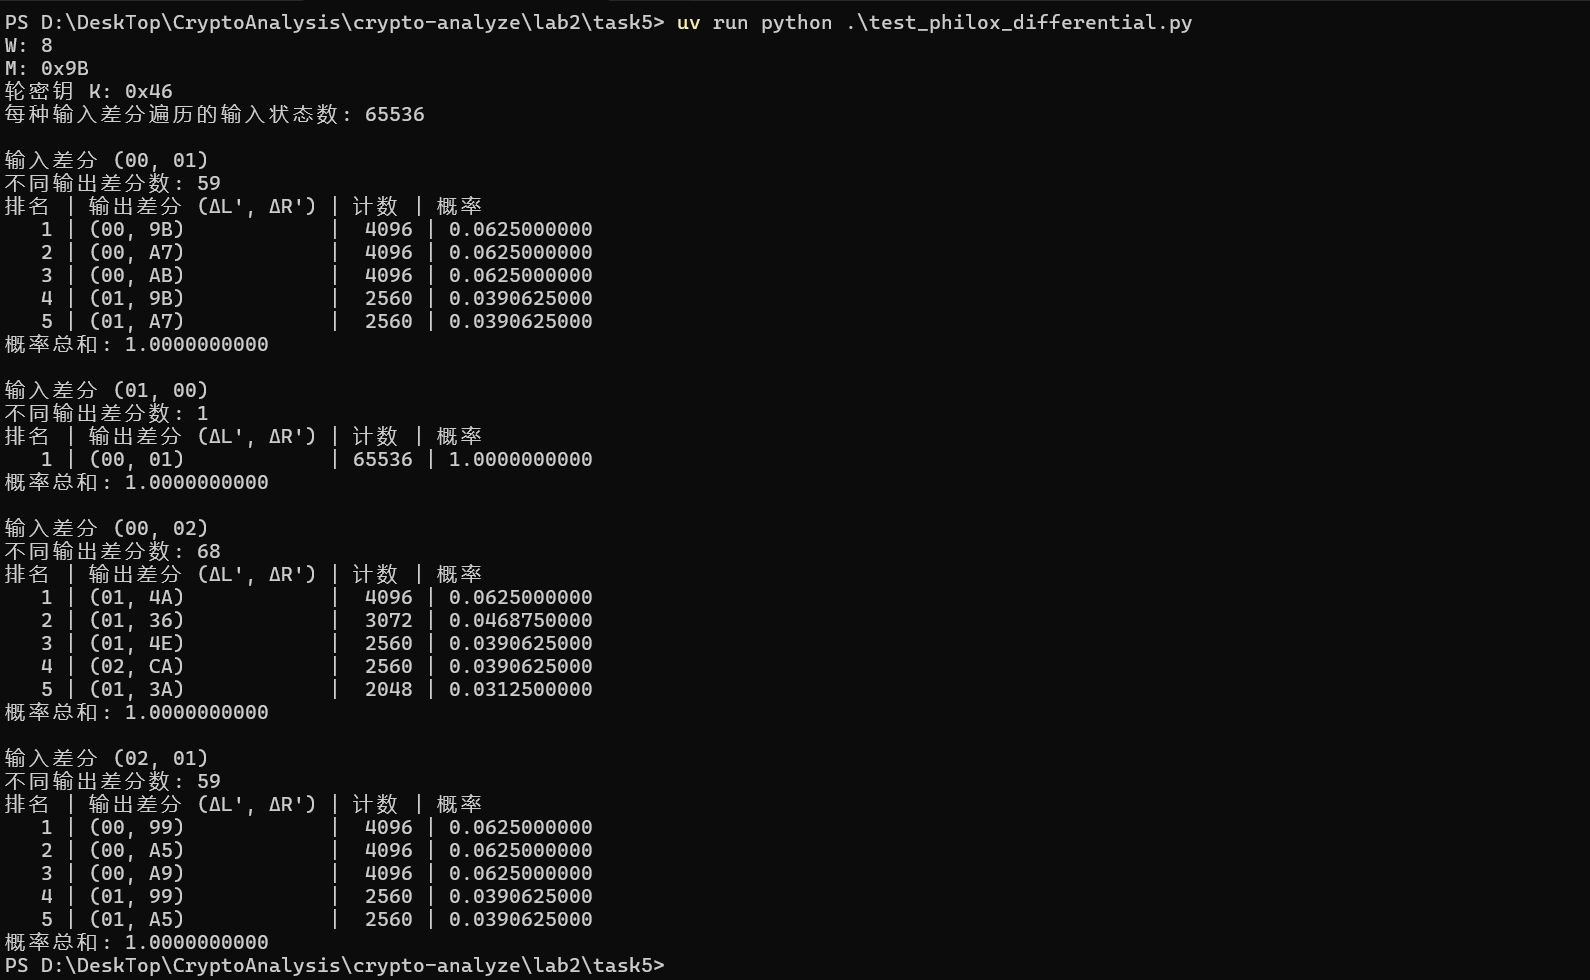
\includegraphics[width=0.96\textwidth]{figures/task5_philow.png}
    \caption{PHILOX-2W一轮差分统计的程序运行结果}
    \label{fig:task5_philox_output}
\end{figure}

\subsection{与随机置换的对比}

随机置换程序先生成包含 $0$ 至 $2^{16}-1$ 的列表，再使用 Python 标准库的洗牌操作将列表重排，得到一个固定种子生成的 16 比特置换。将输入 $(L,R)$ 编码为
\[
    x=(L\ll W)\mathbin{|}R,
\]
然后通过置换表得到 $\pi(x)$，并将其拆分为两个 $W$ 比特分支。程序对所有 $2^{16}$ 个状态及同一组输入差分逐一计数。这里的置换作用于整个 16 比特状态，而不是分别对 $L$、$R$ 两个分支置换。

随机置换只使用状态空间大小和输入差分，不使用 PHILOX 轮函数中的参数 $M$、$K$。参数 $W=8$ 用于确定总状态宽度，并打包、拆分两个分支。随机置换使用固定种子 $20261009$，代码位于
\texttt{lab2/task5/compare\_philox\_random\_permutation.py}。

对于非零输入差分，置换前后的两个状态必不相同，因此随机置换的输出差分不可能为零。对任一固定的非零输出差分 $\beta$，随机置换下的理论平均概率为
\[
    \frac{1}{2^{16}-1}\approx 0.0000152590.
\]
单个随机置换的最高频率可能高于该平均值，这是从 $2^{16}-1$ 种非零输出差分中取最高项后的抽样波动。

图~\ref{fig:task5_random_permutation_output}展示随机置换的运行结果。表~\ref{tab:task5_permutation_comparison}汇总了两种映射在四种输入差分下的输出分布支持数及最高单项概率。随机置换的最高项均为 $12$ 次，即 $12/2^{16}\approx0.0001831$；PHILOX 的最高概率则为 $0.0625$，输入差分 $(\texttt{0x}01,\texttt{0x}00)$ 时为 $1$。此外，随机置换的输出差分分散在约 $2.57$ 万种取值中，而 PHILOX 在本实验中只出现 $1$ 至 $68$ 种输出差分，显示出明显不同的传播分布。

\begin{table}[H]
    \centering
    \scriptsize
    \caption{PHILOX-2W与随机置换的输出差分分布比较}
    \label{tab:task5_permutation_comparison}
    \renewcommand{\arraystretch}{1.15}
    \begin{tabular}{cccrr}
        \toprule
        输入差分 $(\Delta L,\Delta R)$ & PHILOX支持数 & PHILOX峰值概率 & 置换支持数 & 置换峰值概率 \\
        \midrule
        $(\texttt{0x}00,\texttt{0x}01)$ & 59 & 0.0625000000 & 25796 & 0.0001831055 \\
        $(\texttt{0x}01,\texttt{0x}00)$ & 1  & 1.0000000000 & 25824 & 0.0001831055 \\
        $(\texttt{0x}00,\texttt{0x}02)$ & 68 & 0.0625000000 & 25725 & 0.0001831055 \\
        $(\texttt{0x}02,\texttt{0x}01)$ & 59 & 0.0625000000 & 25789 & 0.0001831055 \\
        \bottomrule
    \end{tabular}
\end{table}

随机置换中具体哪些输出差分排在前列由种子决定；本次结果使用固定种子，便于复现。其单次最高项高于理论平均概率 $1/(2^{16}-1)$，是从大量可能的非零输出差分中取最大值所产生的波动。

\begin{figure}[H]
    \centering
    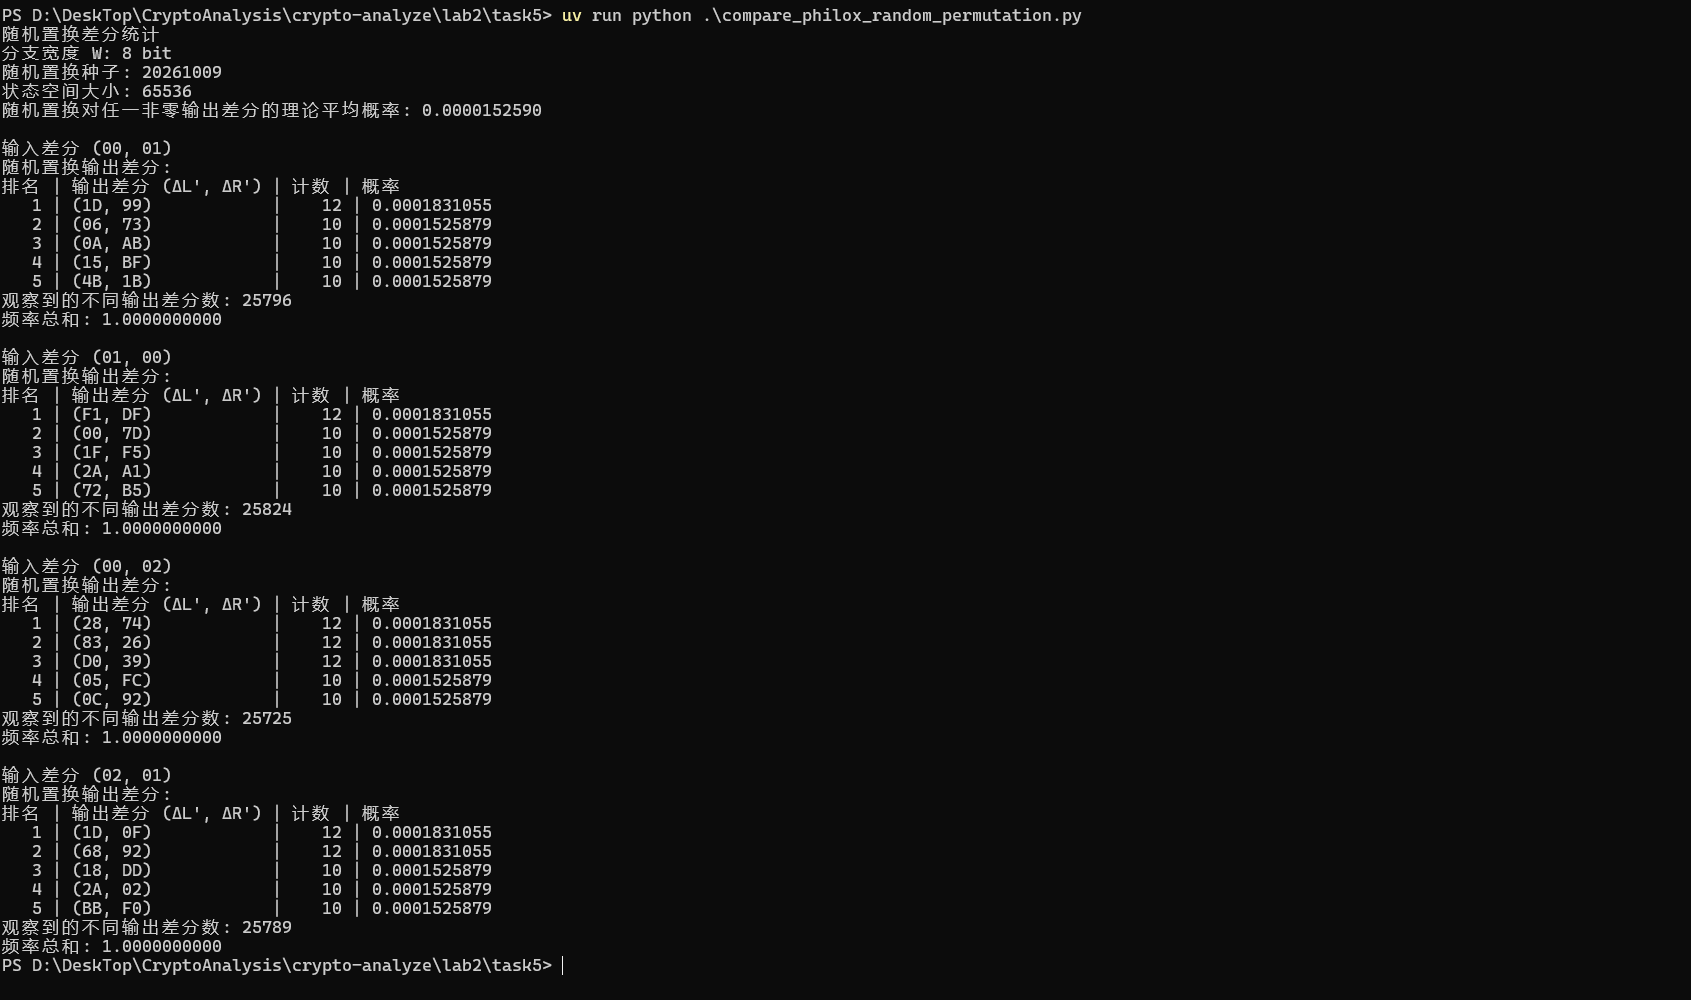
\includegraphics[width=0.96\textwidth]{figures/task5_random_permulation.png}
    \caption{随机置换差分统计及与PHILOX-2W的运行结果对照}
    \label{fig:task5_random_permutation_output}
\end{figure}
